\documentclass[10pt]{beamer}

\usetheme[progressbar=frametitle]{metropolis}
\usepackage{appendixnumberbeamer}
\usepackage[utf8]{inputenc}
\usepackage[T1]{fontenc}
\usepackage[frenchb]{babel}
\usepackage{cmlgc}

\usepackage{booktabs}
\usepackage[scale=2]{ccicons}

\usepackage{pgfplots}
\usepgfplotslibrary{dateplot}

\usepackage{xspace}
\newcommand{\themename}{\textbf{\textsc{metropolis}}\xspace}
\newcommand{\dosion}{\textbf{\textsc{Dosion}}\xspace}

\title{\dosion}
\subtitle{Monitorage faisceaux de moyenne et haute intensité}
%\date{\today}
\date{26 juin 2017}
\author{J.M. Fontbonne, E. Garrido et S. Salvador}
\institute{Jussieu}
\titlegraphic{\hfill
\includegraphics[height=1.5cm]{logo.png}}

\begin{document}

\maketitle

{
\setbeamertemplate{frame footer}{\cite{boissonnat:2017}G. Boissonnat \textit{et al.} \textbf{Characterization and performances of DOSION, a dosimetry equipment dedicated to radiobiology experiments taking place at GANIL.}\textit{NIM,}June 2017}

\begin{frame}[fragile]{Présentation}
\begin{minipage}[h]{.4\linewidth}
\begin{figure}[h]
\begin{center}
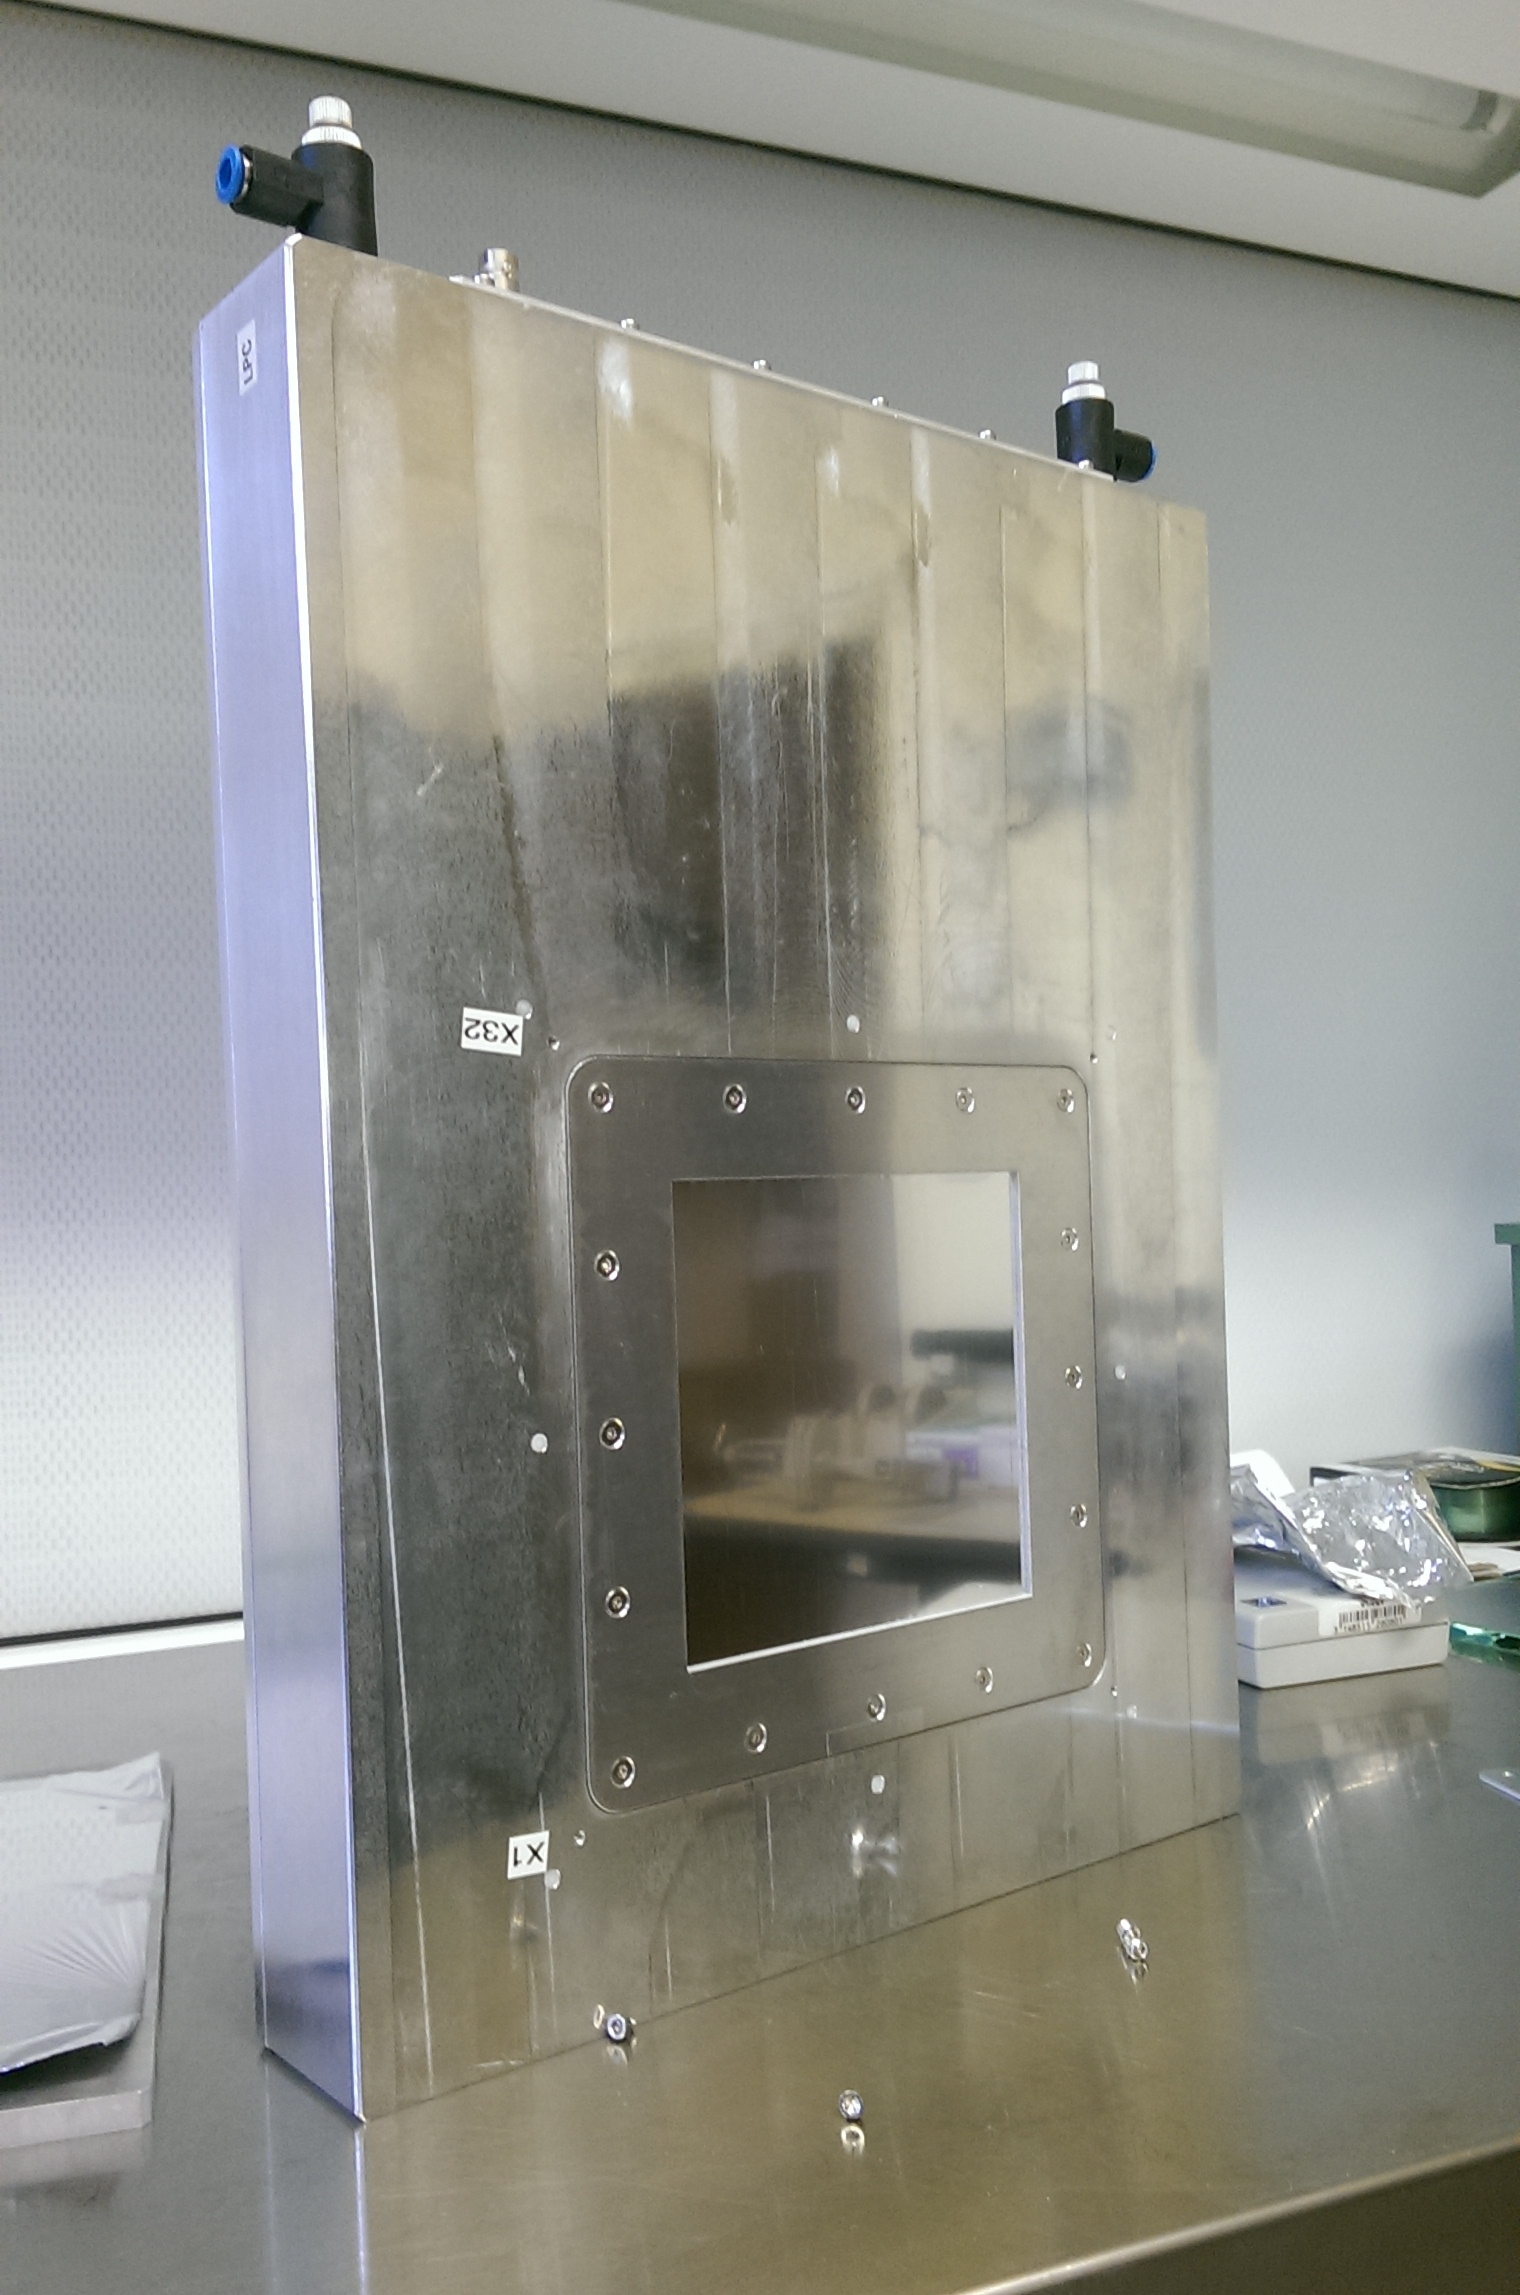
\includegraphics[width=4cm]{Dosion_vert.jpg} 
\end{center}
\end{figure}
\end{minipage}
\hfill
\begin{minipage}[h]{.56\linewidth}
Moniteur faisceau \dosion \textbf{III}\cite{boissonnat:2017} :
\begin{itemize}
\item air à pression ambiante
\item deux chambres d'ionisations :
\begin{itemize}
\item 32 pistes de détection chacune
\item mesures en x et y indépendantes
\end{itemize}
\item surface 9$\times$9 cm$^2$
\item épaisseurs :
\begin{itemize}
\item matériel 6 cm
\item équivalente eau $\simeq$ 100 $\mu$m
\end{itemize}
\end{itemize}
\vspace{1ex}
$\rhd$ FASTER (châssis $\mu$TCA et cartes électromètres)
\end{minipage}
\end{frame}
}

{
\setbeamertemplate{frame footer}{\cite{boissonnat:2015}Thèse de G. Boissonnat, LPC Caen, 2015}
\begin{frame}[fragile]{Caractéristiques}
Des tests ont été conduits pour valider les caractéristiques de \dosion\cite{boissonnat:2015}
\begin{center}
\begin{tabular}{lr}
\hline
Caractéristiques&\hspace{3cm}Résultats\\
\hline
\hline
\'Epaisseur équivalente eau&\alert{$\simeq$100 $\mu$m}\\
Résolution temporelle&\alert{40 $\mu$s à 160 ms}\\
Répétabilité&\alert{<0.1\%}\\
Uniformité de réponse&\alert{1\% (zone active)}\\
Résolution spatiale&\alert{40 $\mu$m}\\
Précision sur la dose&\alert{<5\%}\\
Type de particules&\alert{$\gamma$, e$^-$, hadrons}\\
\hline
\end{tabular} 
\end{center}

\dosion permet également un contrôle en \alert{temps réel}, en natif avec RHB ou en développant sa propre analyse en sortie de FASTER
\end{frame}
}

\begin{frame}[fragile]{Affichage temps réel}
Exemple de graphiques obtenus en temps réel (chaque seconde) avec \alert{RHB}
\begin{figure}[h]
\begin{center}
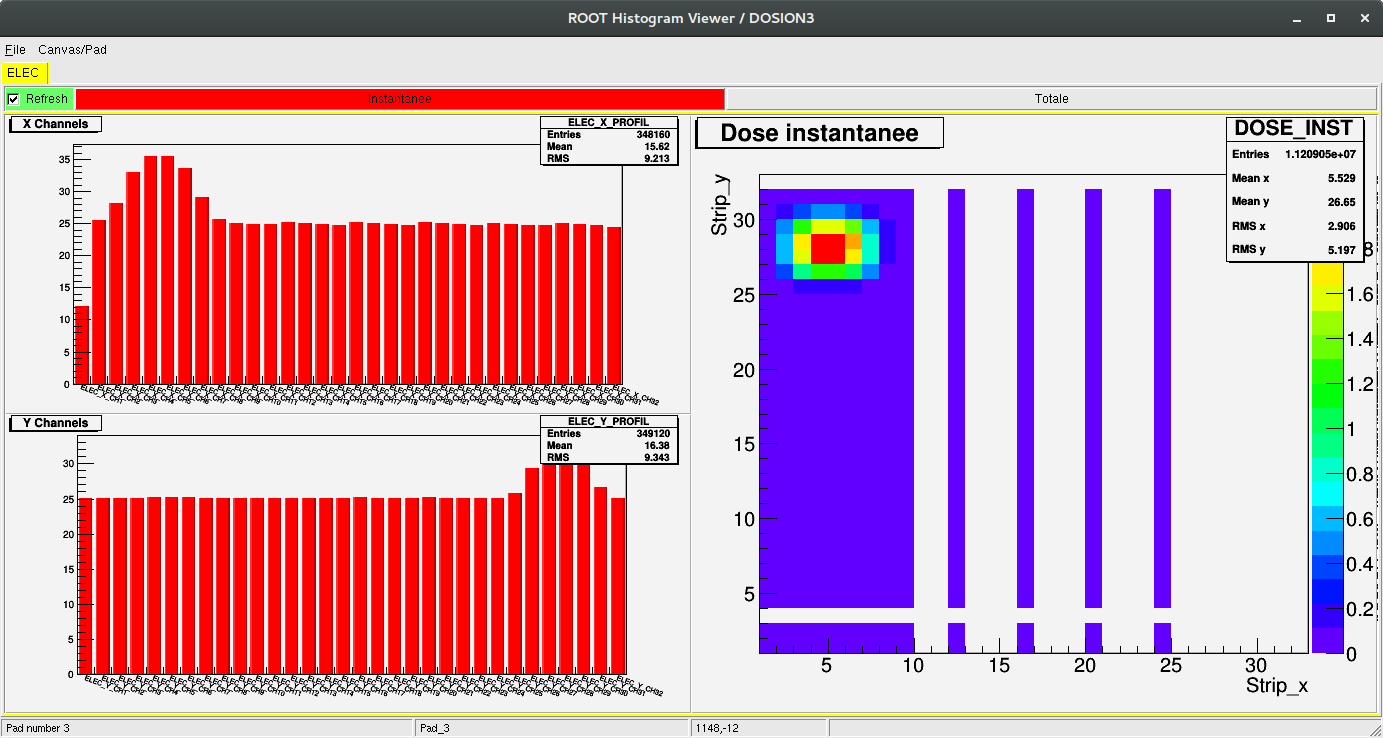
\includegraphics[width=8cm]{RHB.png} 
\end{center}
\end{figure}
$\blacktriangleright$ Un programme d'analyse temps réel plus poussé peut être "raccordé" en sortie directe de FASTER et permettre ainsi un retour sur le contrôle commande de l'accélérateur
\end{frame}

\begin{frame}[fragile]{Analyse post-traitement}
$\rhd$ Les fichiers FASTER obtenus en sortie sont facilement lisibles par d'autres programmes\\
$\rhd$ Ils contiennent pour chaque intégration le $timestamp$ et les 2$\times$32 charges mesurées par les électromètres

\vspace{2ex}
\begin{minipage}[h]{.48\linewidth}
\begin{figure}[h]
\begin{center}
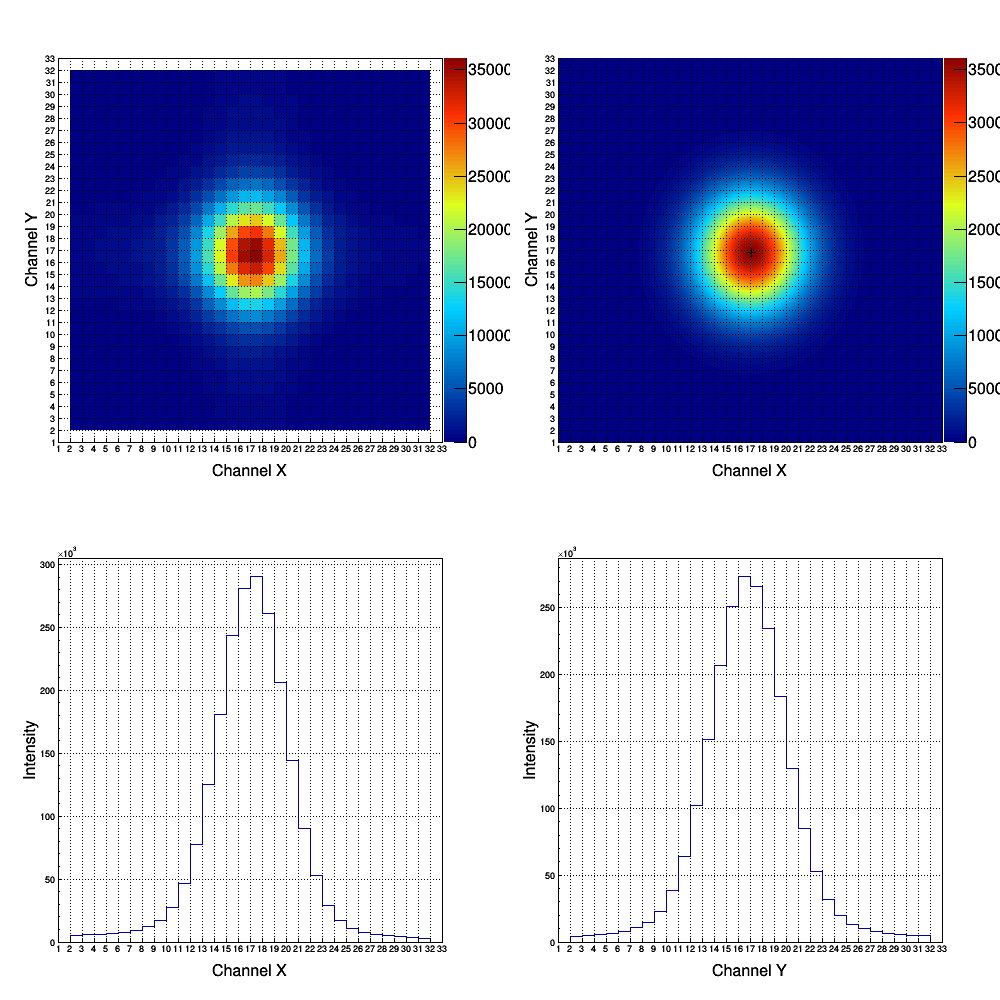
\includegraphics[width=5cm]{Fluence_reconstruction.png}
\end{center}
\end{figure}
\end{minipage}
\hfill
\begin{minipage}[h]{.48\linewidth}
\begin{figure}[h]
\begin{center}
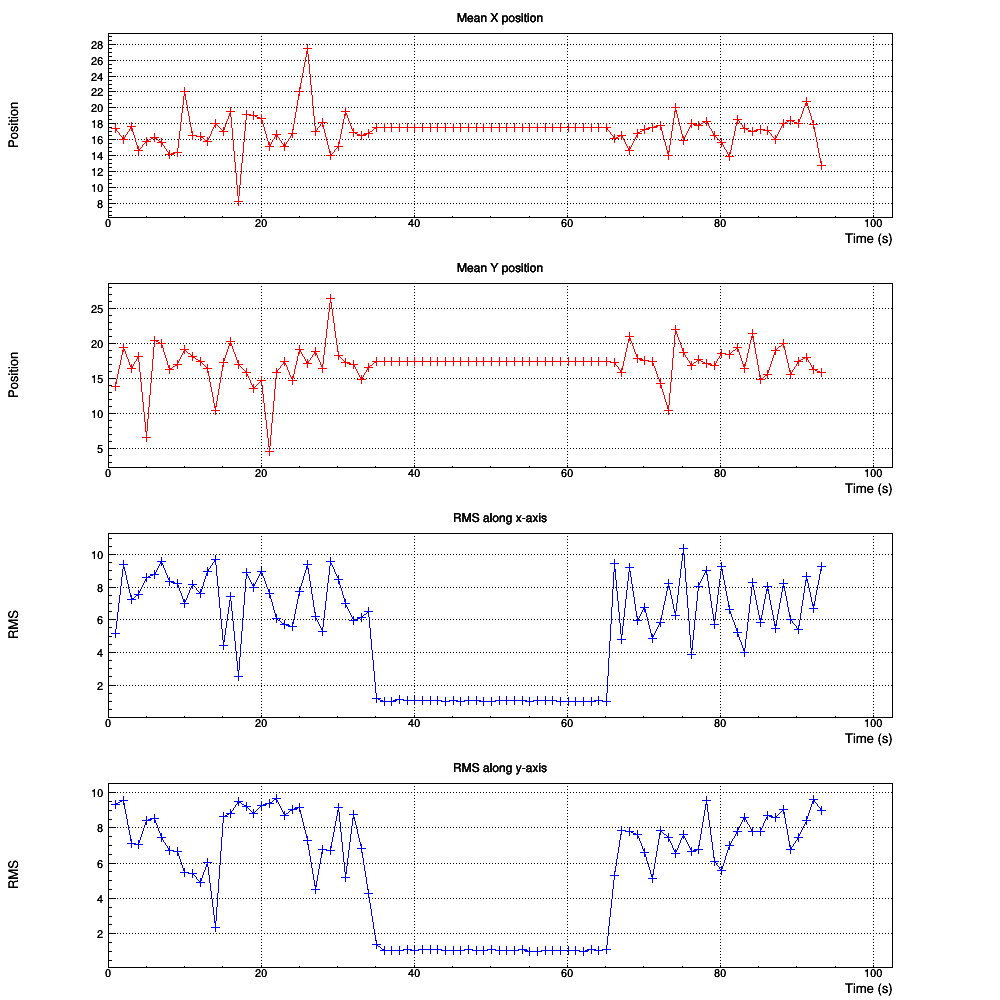
\includegraphics[width=5cm]{Sampling.png}
\end{center}
\end{figure}
\end{minipage}
\end{frame}


\begin{frame}[fragile]{Installations}
\begin{minipage}[h]{.46\linewidth}
\begin{figure}[h]
\begin{center}
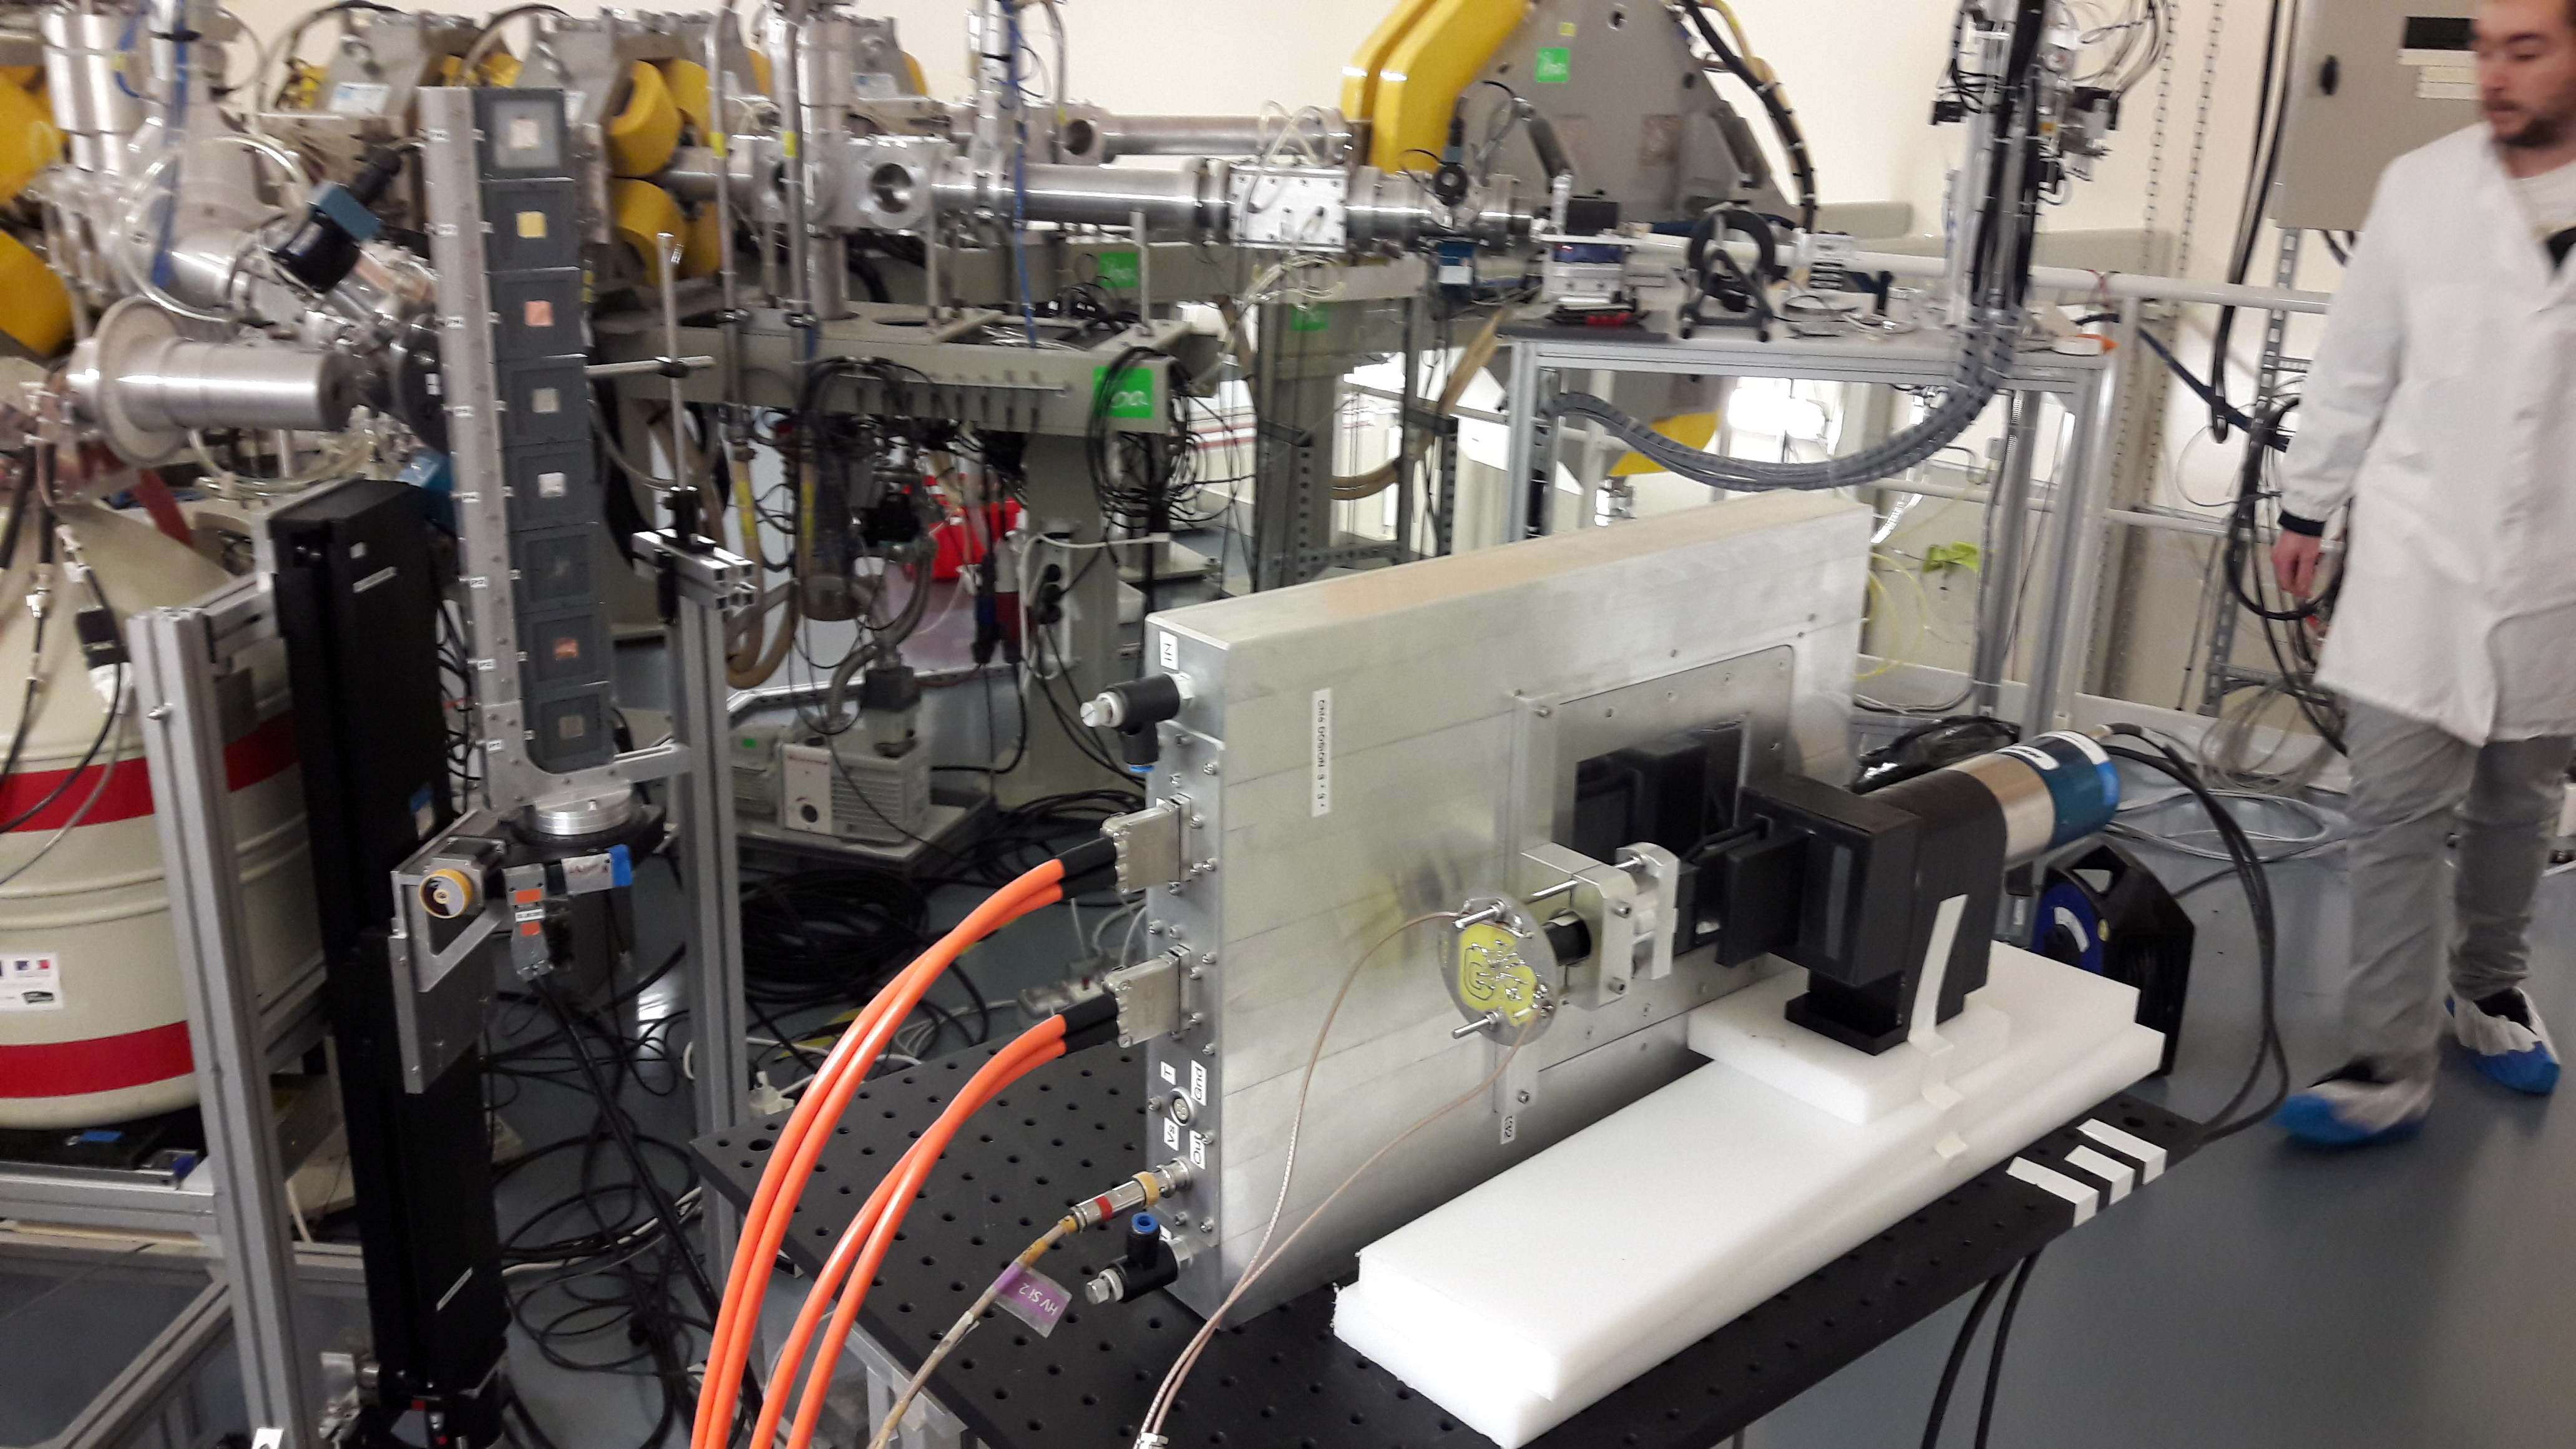
\includegraphics[width=4cm]{Dosion_Arronax.jpg} 
\end{center}
\end{figure}
\end{minipage}
\hfill
\begin{minipage}[h]{.46\linewidth}
\alert{Arronax}, Nantes, février 2017
\end{minipage}

\begin{minipage}[h]{.46\linewidth}
\begin{figure}[h]
\begin{center}
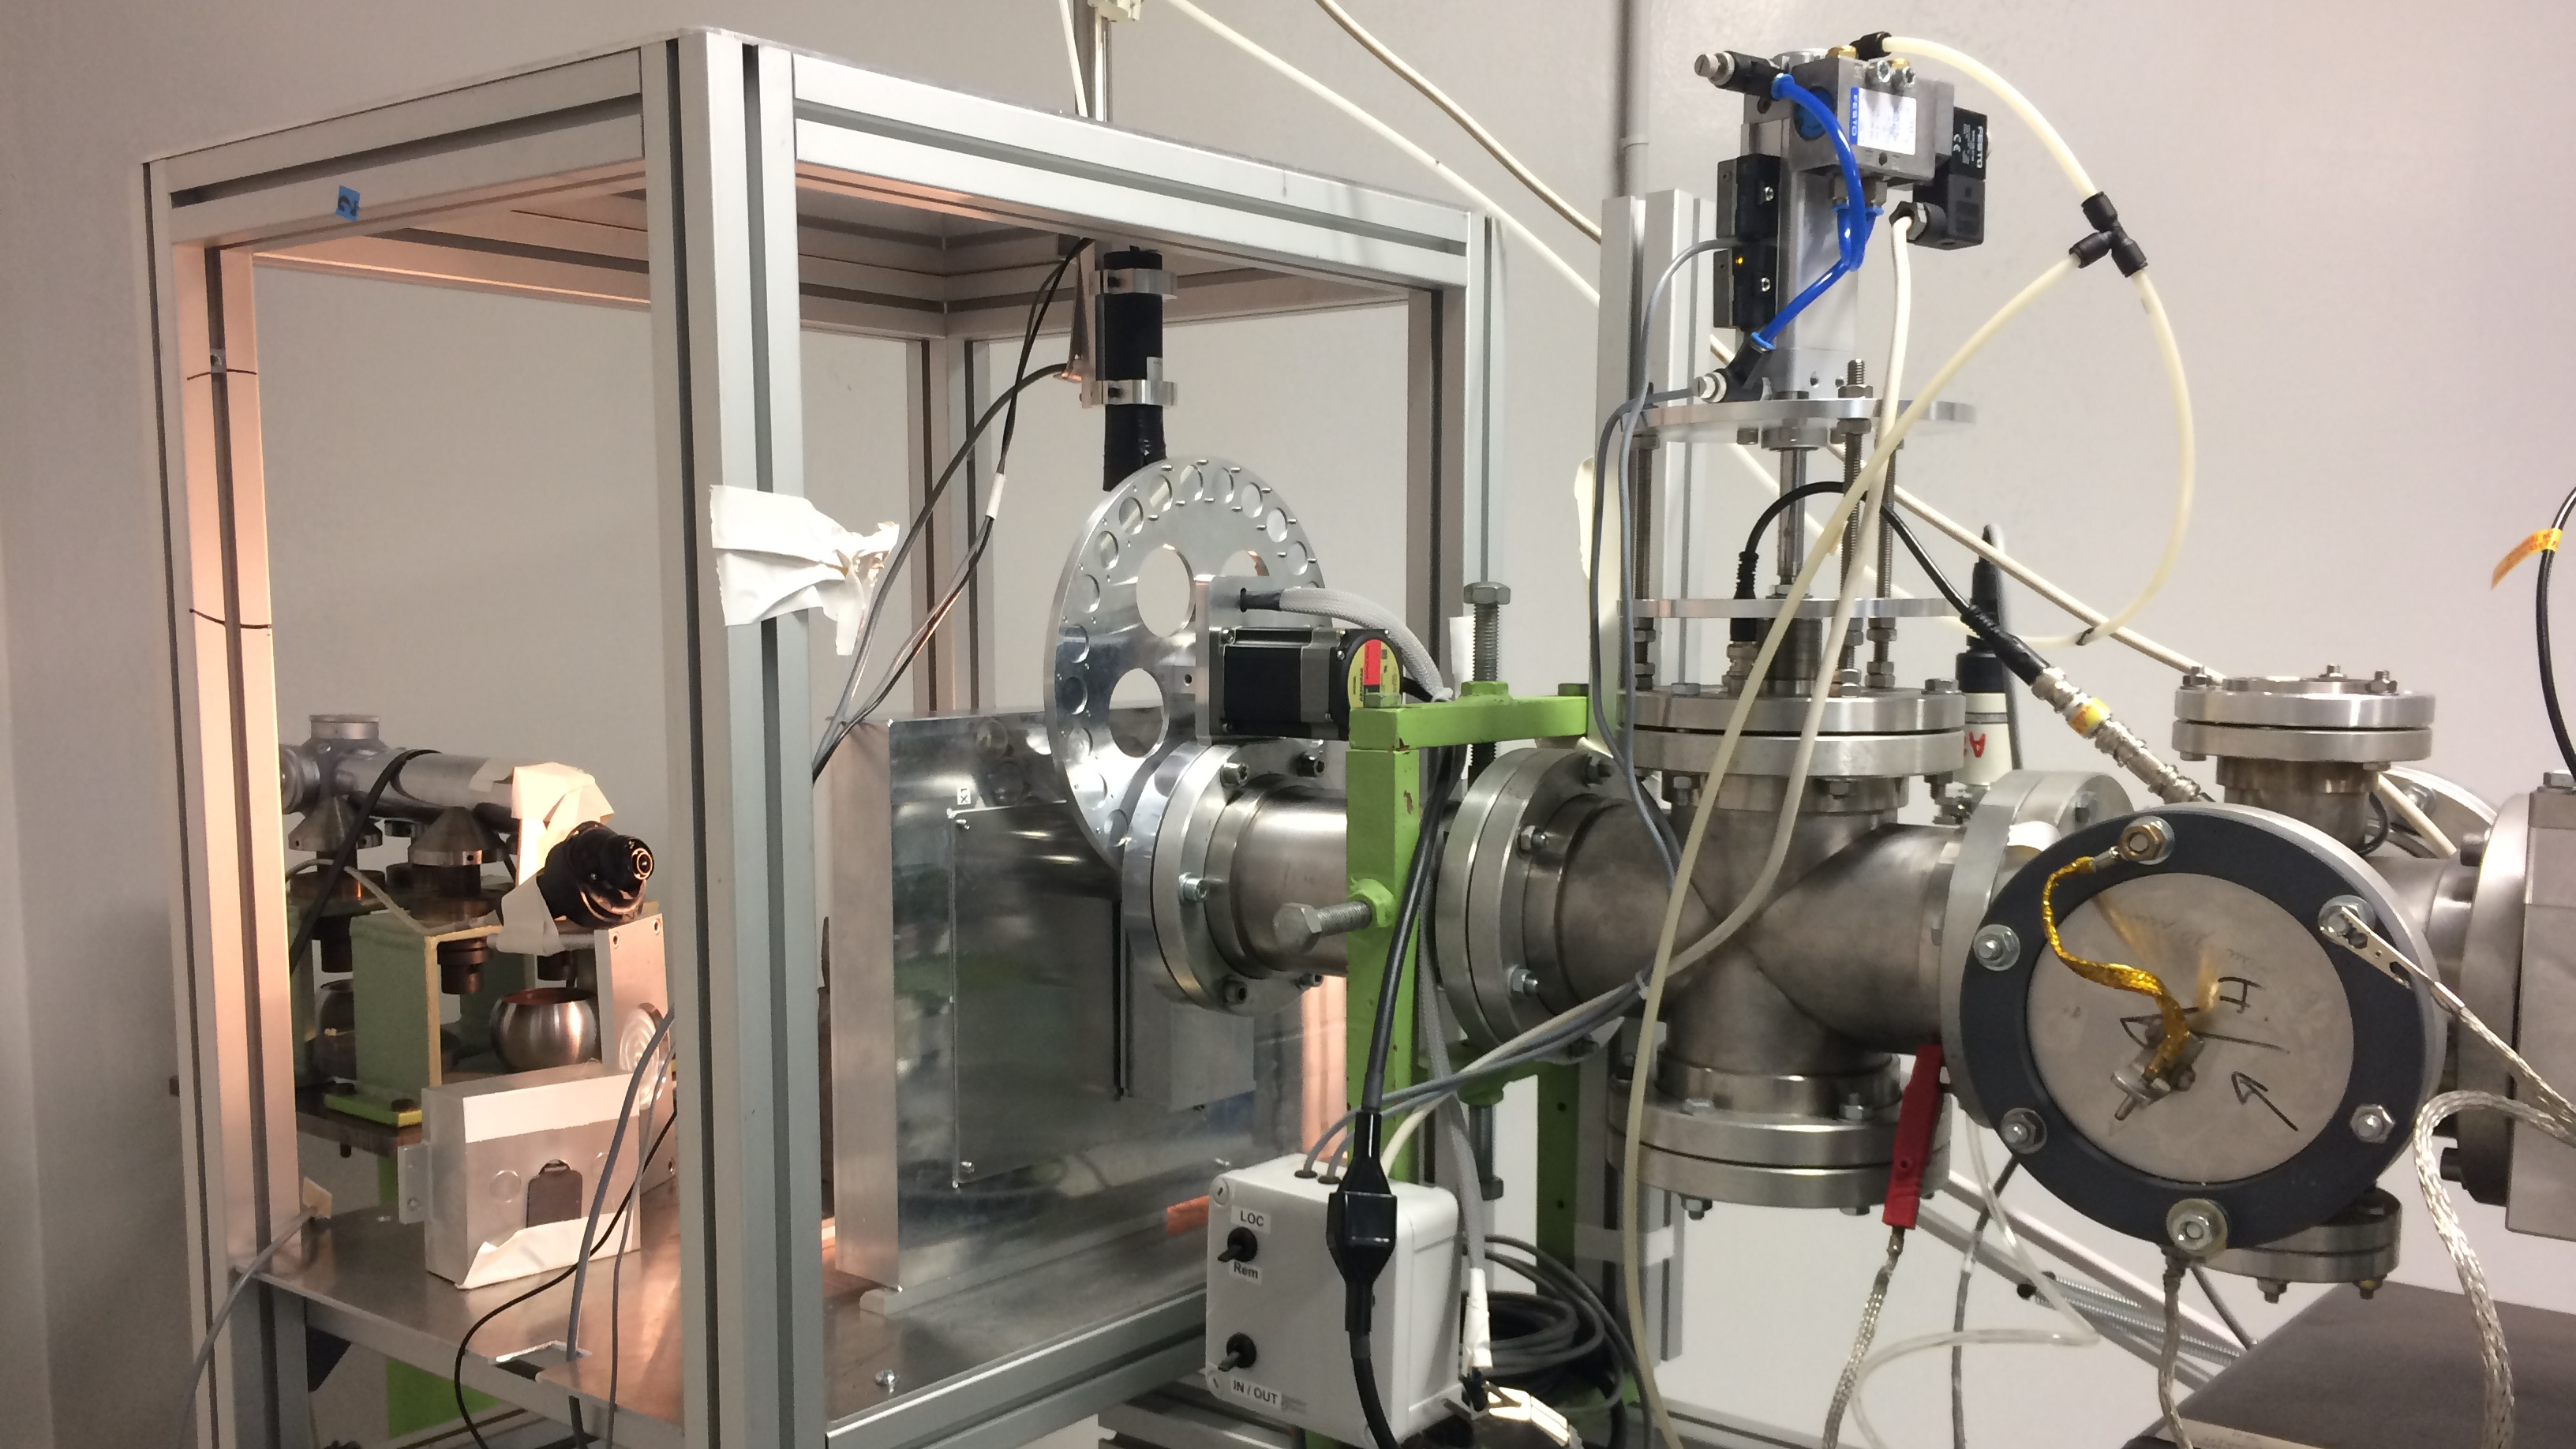
\includegraphics[width=4cm]{Dosion_Cyrce.jpg}
\end{center}
\end{figure}
\end{minipage}
\hfill
\begin{minipage}[h]{.46\linewidth}
\alert{Cyrcé}, Strasbourg, avril 2017
\end{minipage}

\begin{minipage}[h]{.46\linewidth}
\begin{figure}[h]
\begin{center}
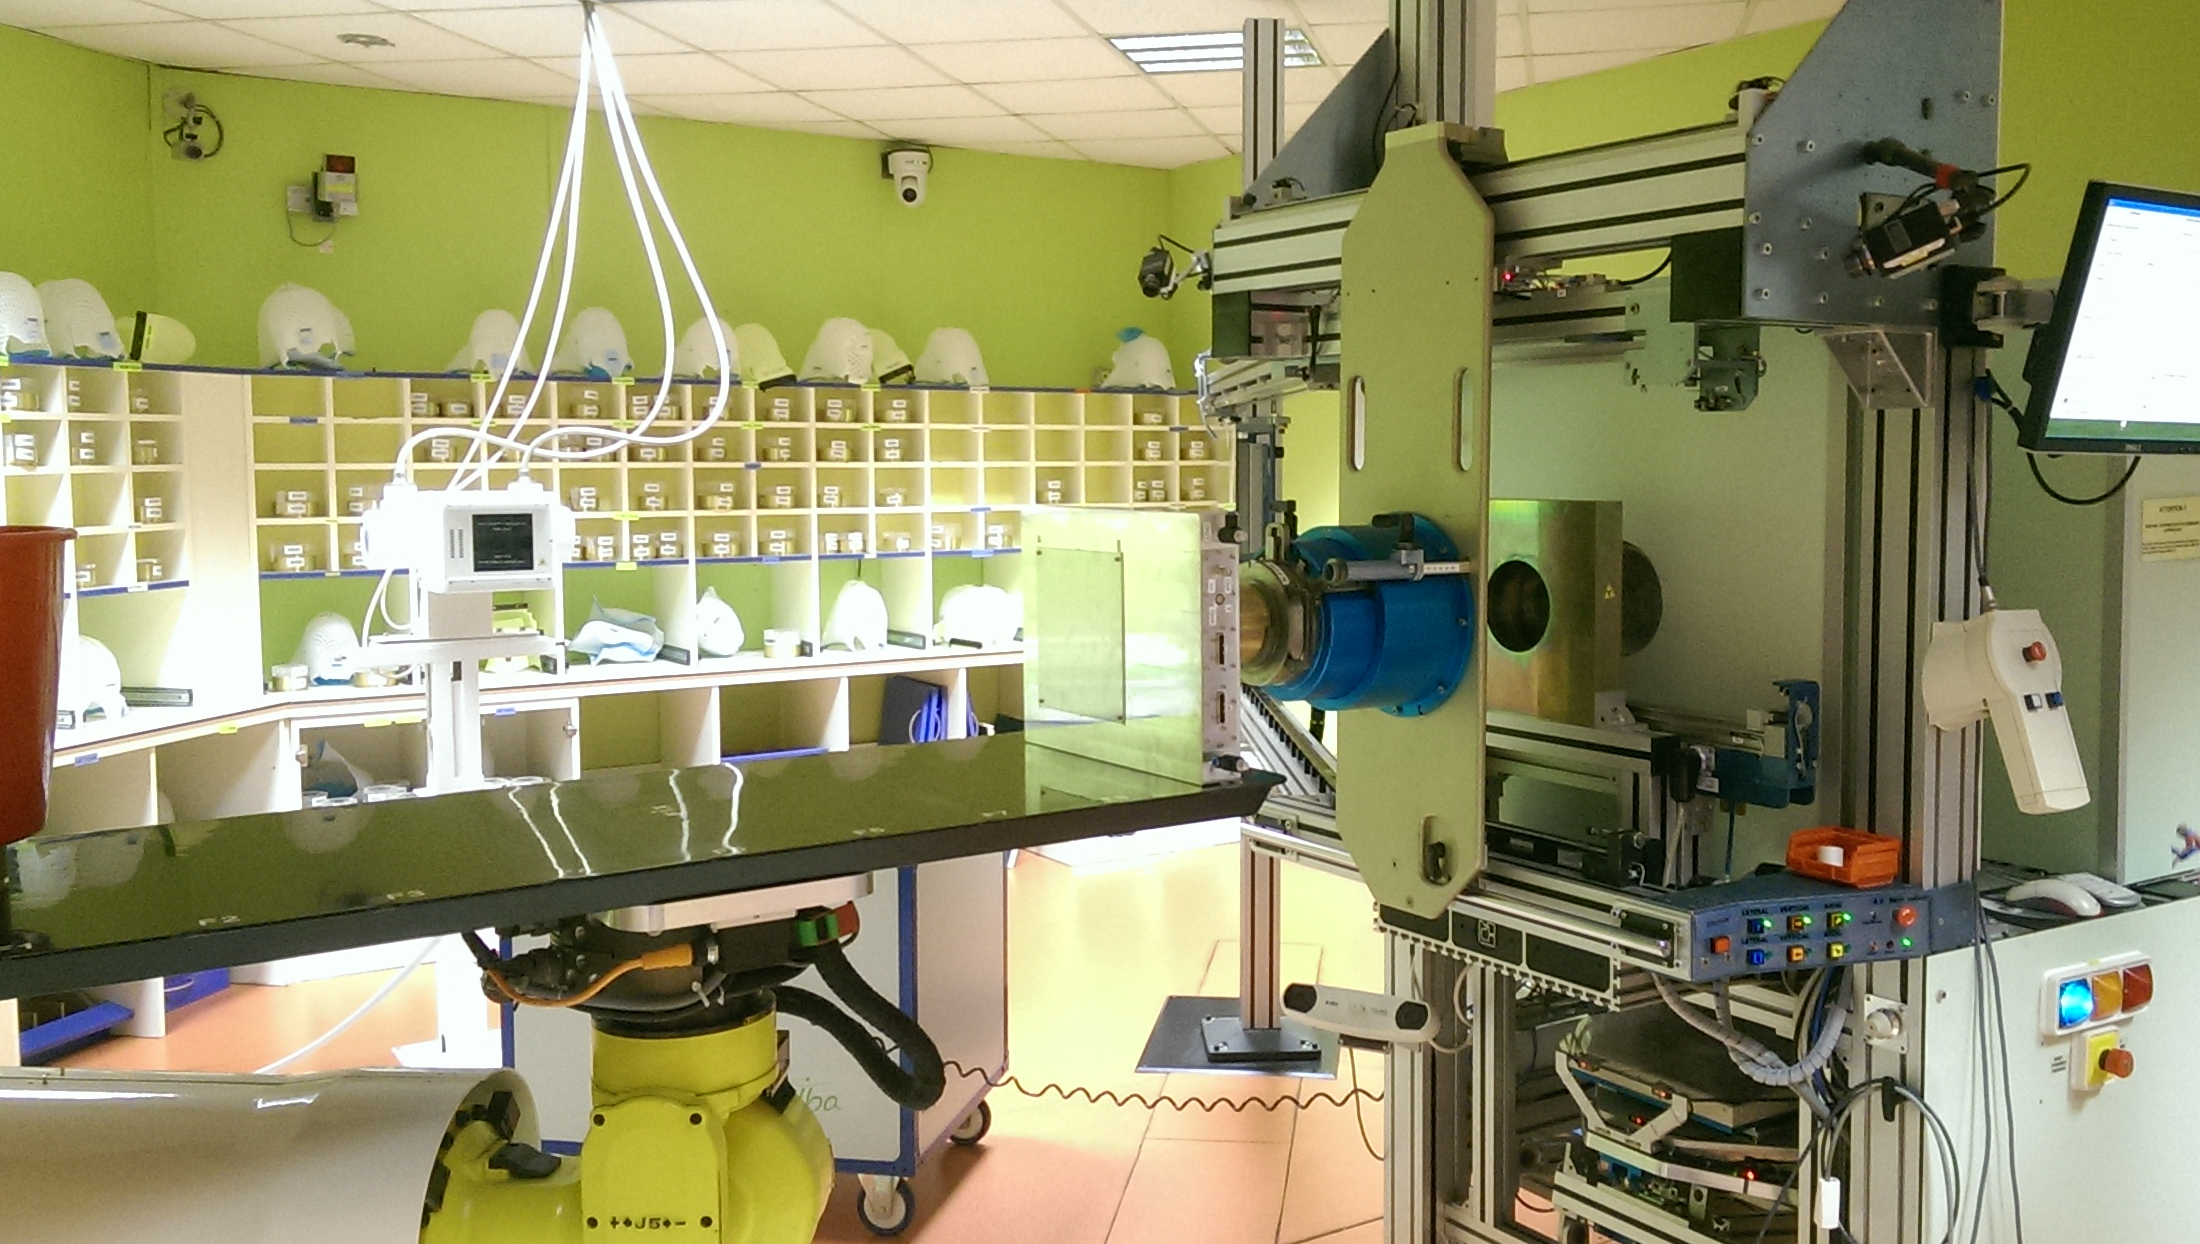
\includegraphics[width=4cm]{Dosion_CPO.jpg}
\end{center}
\end{figure}
\end{minipage}
\hfill
\begin{minipage}[h]{.46\linewidth}
\alert{CPO}, Orsay, mai 2017
\end{minipage}
\end{frame}

\begin{frame}[fragile]{Vers la haute intensité...}
\begin{minipage}[h]{.5\linewidth}
\begin{figure}[t]
\begin{center}
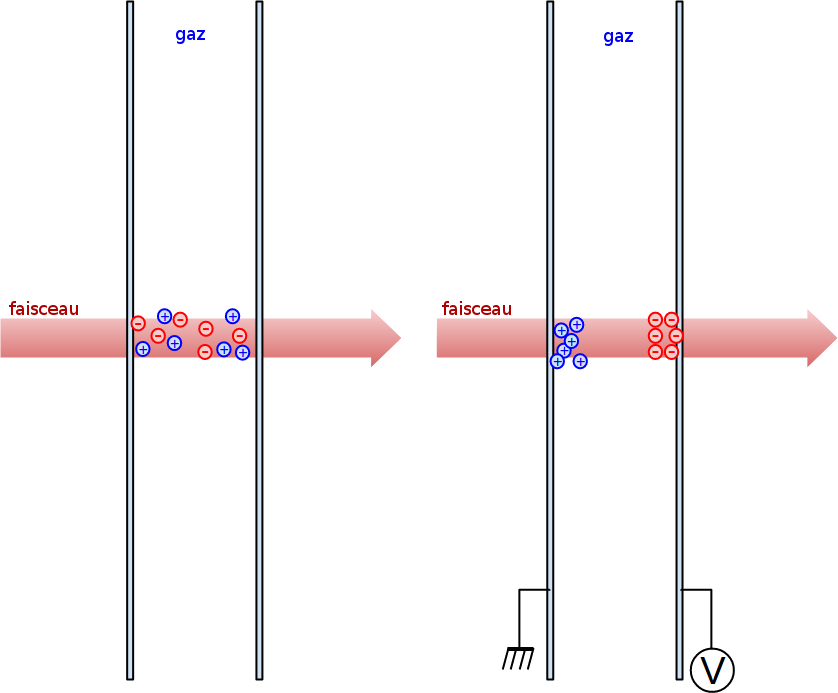
\includegraphics[height=5cm]{IC_bd.png} 
\end{center}
\end{figure}
\end{minipage}
\hfill
\begin{minipage}[h]{.48\linewidth}
\begin{figure}[h]
\begin{center}
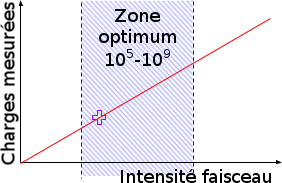
\includegraphics[width=3cm]{Ch_bd.png}
\end{center}
\end{figure}
\vspace{2ex}
Nous calibrons en absolu à basse intensité (<10$^6$part$\cdot$p$^{-1}\cdot$s$^{-1}$) avec un détecteur à scintillation
\end{minipage}

$\blacktriangleright$ Le calibrage n'est valable que si la réponse du détecteur est \alert{linéaire} 
\end{frame}

\begin{frame}[fragile]{Vers la haute intensité...}
\begin{minipage}[h]{.5\linewidth}
\begin{figure}[t]
\begin{center}
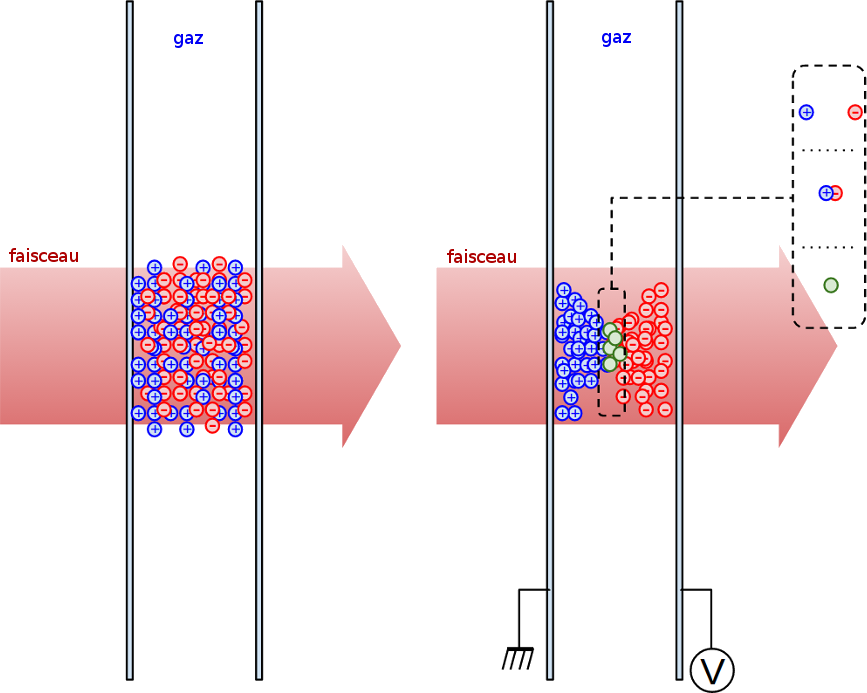
\includegraphics[height=5cm]{IC_hd.png} 
\end{center}
\end{figure}
\end{minipage}
\hfill
\begin{minipage}[h]{.48\linewidth}
\begin{figure}[h]
\begin{center}
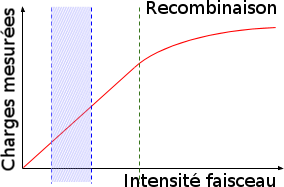
\includegraphics[width=3cm]{Ch_hd.png}
\end{center}
\end{figure}
\vspace{2ex}
Des effets de recombinaisons entre les charges apparaissent à des intensités plus élevées 
\end{minipage}

$\blacktriangleright$ Les électromètres saturent \alert{avant} que les charges ne se recombinent
\end{frame}

\begin{frame}[fragile]{Vers la haute intensité...}
Limite matériel des électromètres à 24 pC/piste
\begin{itemize}
\item changer l'électronique
\item \alert{dériver une partie des charges à la masse}
\end{itemize}
\begin{figure}[h]
\begin{center}
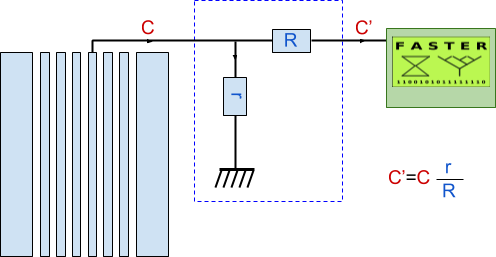
\includegraphics[height=4.2cm]{Deriv.png}
\end{center}
\end{figure}
$\blacktriangleright$ Pas de modifications de \dosion ou de FASTER\\
$\blacktriangleright$ Pas de pertes d'informations
\end{frame}

\begin{frame}[fragile]{...et la très haute intensité}
$\rhd$ Définir la plage de perte de linéarité avant saturation\\
$\rhd$ Vérifier la possibilité de travailler en non-linéarité
\begin{itemize}
\item pouvoir calibrer à ces intensités
\item répétabilité du faisceau
\end{itemize}
\vspace{2ex}
$\rhd$ Modifications matérielles de \dosion
$\left. \text{\parbox{0.48\linewidth}{
\begin{itemize}
\item réduire la taille du gap
\end{itemize}
}} \right.$ $\rightarrow$ limite basse à \alert{1.6 mm}

$\left. \text{\parbox{0.5\linewidth}{
\begin{itemize}
\item changer la nature du gaz
\item changer sa densité
\end{itemize}
}} \right \}$ \alert{étanchéifier} \dosion

$\blacktriangleright$ Implique un développement théorique et des \alert{tests expérimentaux} 
\end{frame}

{\setbeamercolor{palette primary}{fg=black, bg=yellow}
\begin{frame}[standout]
  Questions?
\end{frame}
}

\appendix

\begin{frame}[allowframebreaks]{References}

  \bibliography{Conf_Jussieu}
  \bibliographystyle{unsrt}

\end{frame}

\end{document}
